\documentclass{article}
\usepackage[utf8]{inputenc}
\usepackage[margin=2cm]{geometry}
\usepackage{amsmath}
\usepackage{amsfonts}
\usepackage{amssymb}
\usepackage{graphicx}
\usepackage{amsthm}

\title{Note on Balance Behaviour on the Ecological Dynamical Systems}
\author{Yutong Zhang}
\date{January 2018}

\begin{document}

\maketitle

The \textbf{Lotka–Volterra Equations}, also known as the predator–prey equations, are a pair of first-order, nonlinear, differential equations frequently used to describe the dynamics of biological systems in which two species interact, one as a predator and the other as prey. The populations change through time according to the pair of equations:
$$
\begin{cases}
\displaystyle{\frac{dx}{dt}}=(\alpha-\beta y)x \\
\displaystyle{\frac{dy}{dt}}=(\delta x - \gamma)y
\end{cases}\quad
(\alpha,\beta,\gamma,\delta\geq0)
$$

The Lotka-Volterra Equations shows the equilibrium phenomenon in a isolated ecosystem. Such equilibrium is reflected by the periodicity of the dynamical system. Intuitively, the periodicity could be observed from the following image.
\begin{figure}[!htbp]
    \centering
    \includegraphics[height=13cm]{Lotka-Volterra-VectorPlot.PNG}
    \caption{Equilibrium Behaviour}
    \label{fig:lotka_volterra_vectorplot}
\end{figure}

The actual proof is carried out right below.\pagebreak
\begin{proof}
Represent the tangent of the parametric curve on the $x-o-y$ plane at a point with parameter $t$ with $\displaystyle{\frac{dy}{dx}}$.

On the $x-o-y$ plane, we use secant lines to approach tangent lines -- exactly what we do when defining derivatives. We denote the slope of the tangent lines of the parametric graph of the above equation as $\displaystyle{\frac{dy}{dx}}$ (notice that $\displaystyle{\frac{dy}{dx}}$ is only a notation for convenience, and it is a function of $t$ instead of $x$), and start calculating.
$$
\frac{dy}{dx}=\lim_{\Delta t\to0}\frac{y(t+\Delta t)-y(t)}{x(t+\Delta t)-x(t)}
$$

Now our goal is to prove that
$$
\frac{dy}{dx}=\frac{y'(t)}{x'(t)}
$$
for all $t\neq0$, for which we have two ways to proceed.

First, it is obvious that if $t\neq0$, $x(t+\Delta t)-x(t)\neq0$, since, as the population function, $x$ is defined to be greater than 0 on its domain. Now there are two ways to go:
\begin{enumerate}
\item
$$
\frac{dy}{dx}=\lim_{\Delta t\to0}\frac{y(t+\Delta t)-y(t)}{x(t+\Delta t)-x(t)}=\lim_{\Delta t\to0}\frac{\left(\frac{y(t+\Delta t)-y(t)}{\Delta t}\right)}{\left(\frac{x(t+\Delta t)-x(t)}{\Delta t}\right)}=\frac{\displaystyle{\lim_{\Delta t\to0}}\frac{y(t+\Delta t)-y(t)}{\Delta t}}{\displaystyle{\lim_{\Delta t\to0}}\frac{x(t+\Delta t)-x(t)}{\Delta t}}=\frac{y'(t)}{x'(t)}
$$
Thus proves the goal, and the condition that all the denominators in the previous calculation are not $0$ easily follows from the assumption that $t\neq0$ and $x(t+\Delta t)-x(t)\neq0$, which validates the proof; or, alternatively,
\item
According to \textbf{Cauchy's Mean-Value Theorem}\footnote{Weisstein, Eric W. "Cauchy's Mean-Value Theorem." From MathWorld--A Wolfram Web Resource. http://mathworld.wolfram.com/CauchysMean-ValueTheorem.html}, there exists at least one $\xi\in(t,t+\Delta t)$, such that
$$
\frac{y(t+\Delta t)-y(t)}{x(t+\Delta t)-x(t)}=\frac{y'(\xi)}{x'(\xi)}
$$
for all $\Delta t\neq0$ (which is one of the assumptions of this step of the proof). Now calculate
$$
\frac{dy}{dx}=\lim_{\Delta t\to0}\frac{y(t+\Delta t)-y(t)}{x(t+\Delta t)-x(t)}=\lim_{\Delta t\to0}\frac{y'(\xi)}{x'(\xi)}=\frac{y'(t)}{x'(t)}
$$
Note that in the result of the penultimate step, $\xi$ is a existentially bounded (which means that we acknowledged the existence, typically by reductio ad absurdum, which is exactly how \textbf{Cauchy's Mean-Value Theorem} is proven, but do not know the value itself unless it is proven by construction instead of reductio ad absurdum) variable in the interval $(t,t+\Delta t)$, so it's behaviour is predictable when $\Delta t\to0$: $\xi\to t$, thus validates the last step, which also proves the current step.
\end{enumerate}

Now we have
$$
\frac{dy}{dx}=\frac{y'(t)}{x'(t)}=\frac{(\delta x-\gamma)y}{(\alpha-\beta y)x}
$$
We proceed by first integrate with respect with $x$.
\begin{align*}
\frac{dy}{dx}&=\frac{(\delta x-\gamma)y}{(\alpha-\beta y)x}\\
\frac{(\alpha-\beta y)}{y}\frac{dy}{dx}&=\frac{(\delta x-\gamma)}{x}\\
\int\frac{(\alpha-\beta y)}{y}dy&=\int\frac{(\delta x-\gamma)}{x}dx\\
\alpha\ln\lvert y\rvert-\beta y+C_1&=\delta x-\gamma\ln\lvert x\rvert+C_2
\end{align*}
Now merge the integration constants $C_1$ and $C_2$, and eliminate the absolute value since $x,y>0$.
$$
\alpha\ln y-\beta y=\delta x-\gamma\ln x+C
$$
which will be (we denote $e^C$ with a new constant $K>0$)
$$
\frac{x^\gamma}{e^{\delta x}}\cdot\frac{y^\alpha}{e^{\beta y}}=K
$$
Now we denote
$$
f(x)=\frac{x^\gamma}{e^{\delta x}}\mathrm{\quad and\quad}g(y)=\frac{y^\alpha}{e^{\beta y}}
$$
The parametric curve $(x(t),y(t))$ on the $x-o-y$ plane will now satisfy the following property.
$$
f(x)g(y)=K
$$
Now take the derivative of each function of $f(x)$ and $g(y)$. (it is confusing but now $x$ and $y$ are independent variables instead of function, so do not mix it up with the previous $x(t)$ and $y(t)$)
\begin{align*}
\frac{\partial}{\partial x}\frac{x^{\gamma }}{e^{\delta  x}}&=x^{\gamma -1} e^{\delta  (-x)} (\gamma -\delta  x)\\
\frac{\partial}{\partial y}\frac{y^\alpha}{e^{\beta  y}}&=y^{\alpha-1} e^{\beta  (-y)} (\alpha-\beta  y)
\end{align*}
Now solve for stationary points
\begin{align*}
x&=\frac{\gamma}{\delta}\mathrm{\quad for\quad}\gamma,\delta\neq0\\
y&=\frac{\alpha}{\beta}\mathrm{\quad for\quad}\alpha,\beta\neq0
\end{align*}

Now visualize the graph of $f(x)$.
\begin{figure}[!htbp]
    \centering
    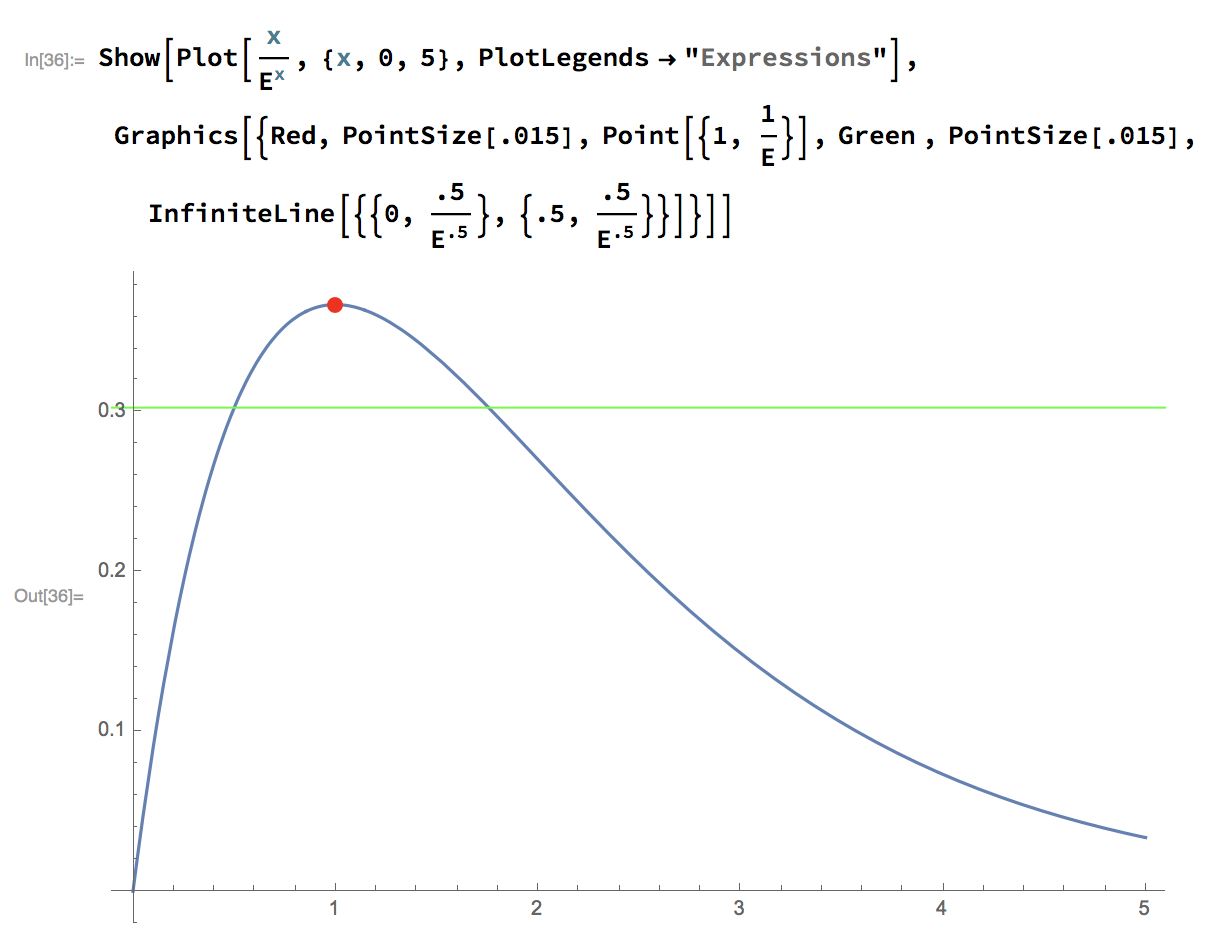
\includegraphics[height=11.5cm]{Lotka-Volterra-ComponentX.png}
    \caption{Visualization of $f(x)$}
    \label{fig:lotka_volterra_componentx}
\end{figure}
From the graph and the derivative of $f(x)$, the following qualitative properties could be induced:\footnote{All properties qualitative could be deducted quantitatively from the basic properties of $f(x)$ and $f'(x)$, but due to the existence of the deadline, such trivial part of the thesis is thus omitted. If necessary, please contact knight.of.lambda.calculus@gmail.com, thank you.}
\begin{enumerate}
\item The function $f(x)$ has a extreme value point, aka a local maximum, at $x=\displaystyle{\frac{\alpha}{\beta}}$\footnote{So does function $g(y)$, but the proof is symmetric at this point thus omitted.};
\item The function $f(x)$ is monotonically increasing over the interval $\displaystyle{\left(0,\frac{\alpha}{\beta}\right)}$ and monotonically decreasing ovwer the interval $\displaystyle{\left(\frac{\alpha}{\beta},+\infty\right)}$;
\item $$\lim_{x\to0}f(x)=0\mathrm{\quad and\quad}\lim_{x\to+\infty}f(x)=0$$i.e. $y=0$ is the horizontal asymptote of $f(x)$; and
\item $\forall x>0.\,f(x)>0$.
\end{enumerate}
We denote $\displaystyle{M_x=f(\frac{\alpha}{\beta})\mathrm{\quad and\quad}M_y=g(\frac{\gamma}{\delta})}$. Now we perform case analysis on the value of $K$.
\begin{itemize}
\item $K\in\mathbb{R}\setminus\left(0,M_x\cdot M_y\right
]$: Impossible, trivial;
\item $K=M_x\cdot M_y$: The differential dynamical system has a unique solution at P
$$
\begin{cases}
x=\frac{\alpha}{\beta}\\
y=\frac{\gamma}{\delta}
\end{cases}
$$
thus the unstable equilibrium point.
\item $K\in\left(0,M_x\cdot M_y\right)$:
Denote $s=\displaystyle{\frac{K}{M_y}}$, and then it is trivial that $s\in(0,M_x)$. Now the equation $f(x)=s$ will have to unequal solution, denoted as $x_{\min}$ and $x_{\max}$, from the observation made in the graph and also the quantitative and qualitative analysis made of the differential dynamical system. Now for any given $K$ such two $x_{\min}$ and $x_{\max}$ are fixed, thus perform case analysis on the value of $x$:
\begin{itemize}
\item
For any $x$ out side of the interval $[x_{\min},x_{\max}]$ there will not be a solution, i.e. no point on the graph, because from the observation, $f(x)<s$ in such cases, thus
$$
f(x)\cdot g(y)<s\cdot g(y)\leq s\cdot M_y=K
$$
\item
If $\displaystyle{x\in\left(x_{\min},x_{\max}\right)}$, from the observation and analysis, $f(x)>s$, thus there will be an equation
$$
g(y)=\frac{K}{f(x)}
$$
for any such $x$. And since
$$
g(y)=\frac{K}{f(x)}<\frac{K}{s}<M_y
$$
the equation will have two unique solution.
\item
If $x\in\{x_{\min},x_{\max}\}$, then $f(x)=s$, thus
$$
f(x)\cdot g(y)=K\implies g(y)=M_y
$$
will have only one solution (of multiplicity $2$) $y=\displaystyle{\frac{\gamma}{\delta}}$.
\end{itemize}
\end{itemize}

\begin{figure}[!htbp]
    \centering
    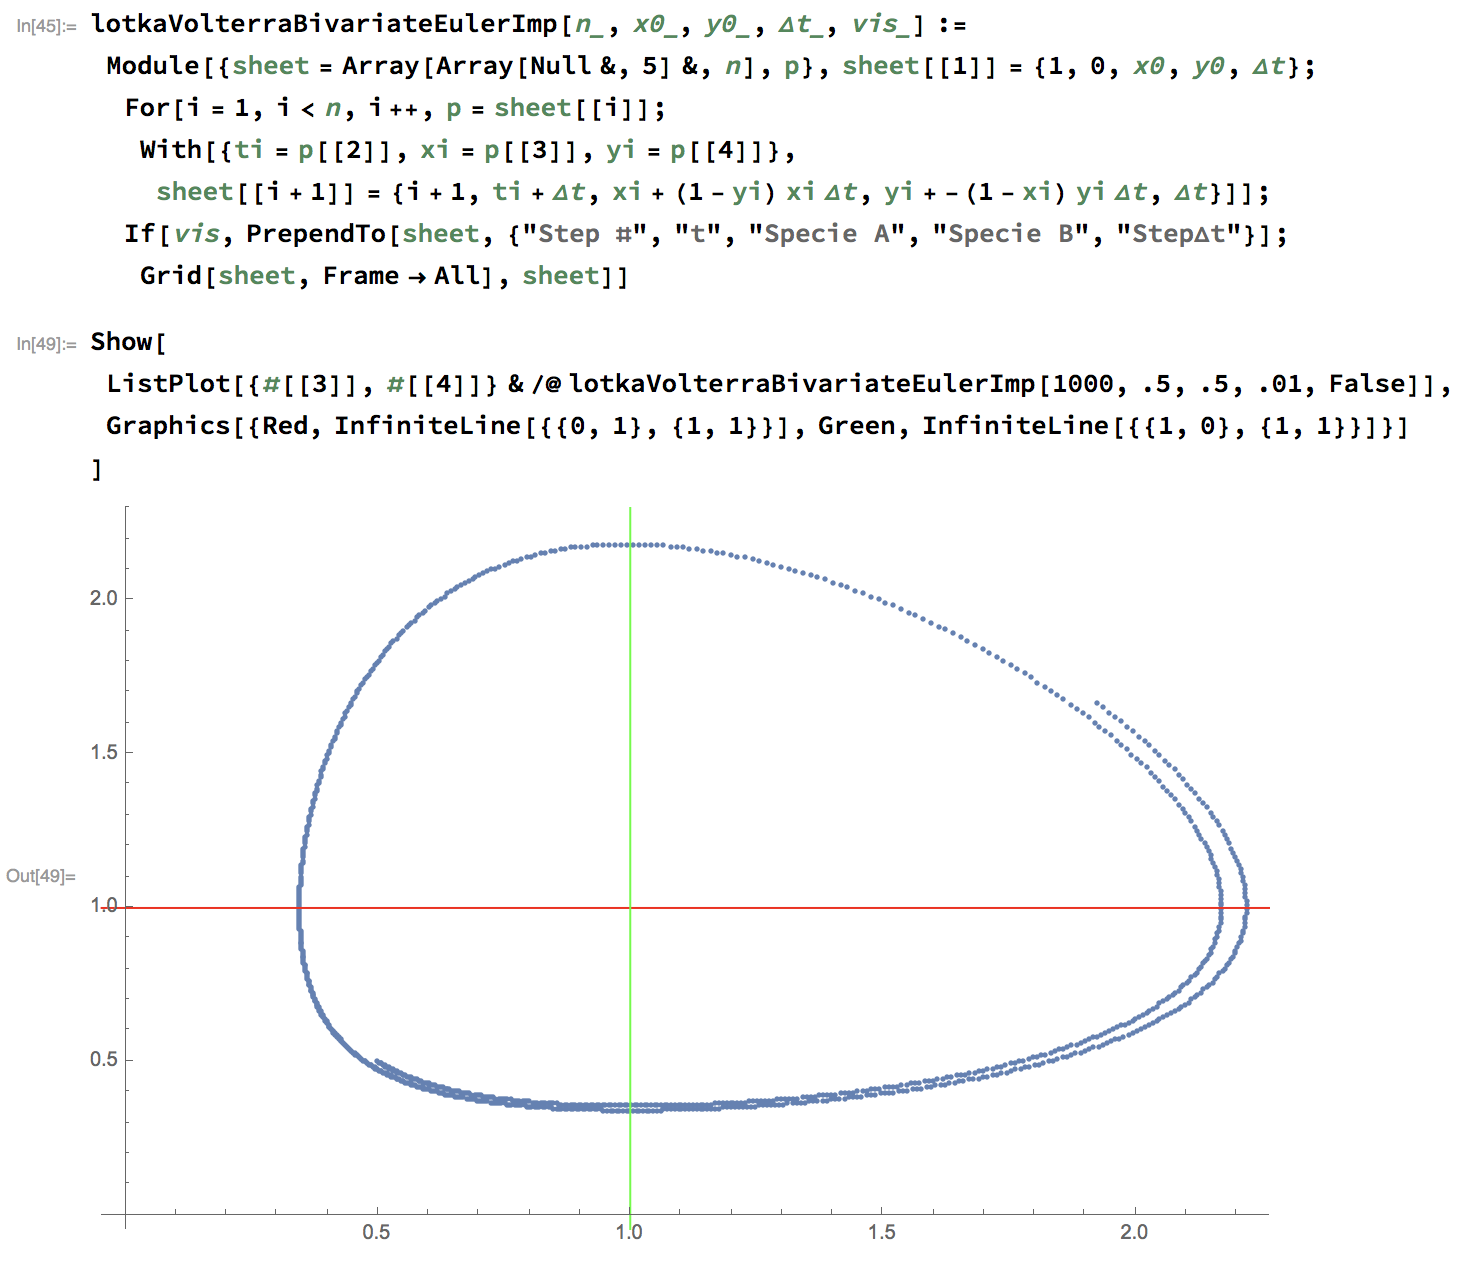
\includegraphics[height=10cm]{Lotka-Volterra-Vertex.png}
    \caption{Equilibrium Vertex Visualization}
    \label{fig:lotka_volterra_vertex}
\end{figure}
Now the properties stated above together with Figure \ref{fig:lotka_volterra_vertex}, we can deduce that for each $K$, there will be a \textbf{equilibrium trajectory} or a \textbf{equilibrium point} (though the latter is highly unlikely to happen in natural data), and together with the assumption that
$$
x(t)\in\mathbf{D}^n(I)
$$
$$
y(t)\in\mathbf{D}^n(I)
$$
up to a sufficient $n$-th order with an appropriate domain $I$, the statement that the \textbf{Lotka-Volterra Equations} are de facto \textbf{Equilibrium Trajectory} with \textbf{periodicity is proven.}
\end{proof}

\end{document}
